\documentclass{beamer}
\usepackage[utf8]{inputenc}
\usepackage[francais]{babel}
\usepackage[T1]{fontenc}
\usepackage{amsmath}
\usepackage{amsfonts}
\usepackage{amssymb}
\usepackage{graphicx}
\usepackage{tikz}
\usetikzlibrary{arrows}
\usepackage[squaren,Gray]{SIunits} % Physical units rendering
\usepackage{sistyle}
\usepackage[autolanguage]{numprint}
%\usepackage{xfrac}
\usepackage{bm}
\usepackage{color} % Colors in text
\usepackage[version=3]{mhchem} % Chemical reactions
\usetheme{CambridgeUS}
\setbeamercolor{title}{bg=red!65!black,fg=white}

\setbeamertemplate{sidebar right}
{
  \vfill%
  \llap{\insertlogo\hskip0.1cm}%
  \vskip2pt%
  \llap{\href{http://tex.stackexchange.com/}{A link to tex.sx}\hskip0.2cm}% NEW
  \vskip3pt% NEW
  \llap{\usebeamertemplate***{navigation symbols}\hskip0.1cm}%
  \vskip2pt%
}

\begin{document}

\title{Synthèse de l'ammoniac}
\author{Groupe 1254}
\institute[UCL]{Ecole polytechnique de Louvain-la-neuve}
\date{}
\maketitle
%==========================================================
\begin{frame}{Démarche suivie}
\begin{center}
Nous allons vous présenter:
	\begin{enumerate}
	\item La tâche 3: Etude environnementale
	\item La tâche 8: Comment diminuer notre rejet en \ce{CO2} ?
		\begin{itemize}
		\item L'électolyse
		\item Le Biogaz
		\item Les Algues
		\end{itemize}
	\end{enumerate}
\end{center}
\end{frame}

\begin{frame}{Aspects énergétique}
\begin{center}
Points d'entrée et de sorties:
\begin{itemize}
\item Four à méthane
\item Condensation du \ce{CO2} et de l'\ce{H2O}
\item Refroidissement du réacteur à \ce{NH3}
\item Condensation de l'ammoniac
\end{itemize}

Amélioration possible:
\begin{itemize}
\item Réutilisation de l'eau rejetée
\end{itemize}
\end{center}
\end{frame}

\begin{frame}{Rejets \ce{CO2}}
\begin{center}
\part*{Sources}
\begin{itemize}
\item Four à méthane: \unit{207}{t} de \ce{CO2}.
\item Réformeur primaire + Réformeur secondaire + Water-gas shift: \unit{1718}{t} \ce{CO2}.
\end{itemize}
\part*{Solutions}
\begin{itemize}
\item Autre source d'hydrogène
\item Le biogaz
\item Capturer et stocker le \ce{CO2}
\end{itemize}
\end{center}
\end{frame}

\begin{frame}{Electrolyse de l'eau}
\begin{columns}
\begin{column}{0.40\textwidth}
$$ \ce{2H2O_{(l)} <=> 2H2_{(g)} + O2_{(g)}}$$
 
Principaux avantages:
\begin{itemize}
\item Pas de rejet de \ce{CO2}
\item Coûts de transport diminués
\end{itemize}
\end{column}
\begin{column}{0.40\textwidth}
\begin{figure}
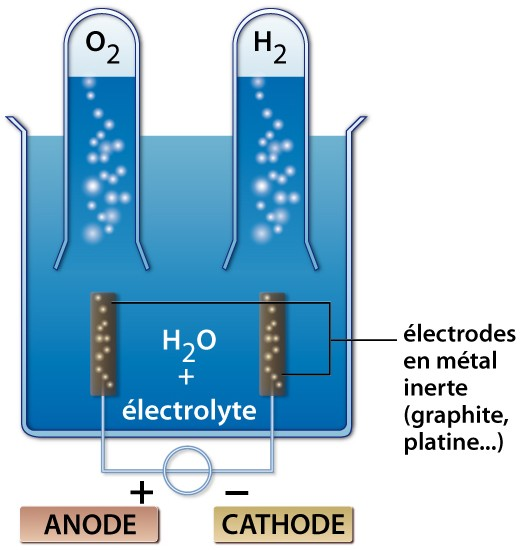
\includegraphics[scale=0.25]{schema/electrolyse}
\end{figure}
\end{column}
\end{columns}
\end{frame}

\begin{frame}{Electrolyse de l'eau}
\part*{Puissance requise pour produire 1500 [tonnes/jour] d'ammoniac}
\begin{itemize}
\item $\simeq$ \textbf{5.7 [GW]}
\item $\Rightarrow$ 4 réacteurs nucléaires (d'une puissance de 1.5 [GW])
\item $\Rightarrow$ 2850 Ha de panneaux photovoltaïques (avec un rendement de 20 \% pour un rayonnement d'une intensité 1000 [W/$m^2$])
\end{itemize}
\part*{Principaux désavantages}
\begin{itemize}
\item Consommation d'électricité
\item Stockage de l'hydrogène
\item Dangerosité de l'hydrogène
\end{itemize}
\end{frame}



\begin{frame}{Biométhanisation}
\begin{figure}
		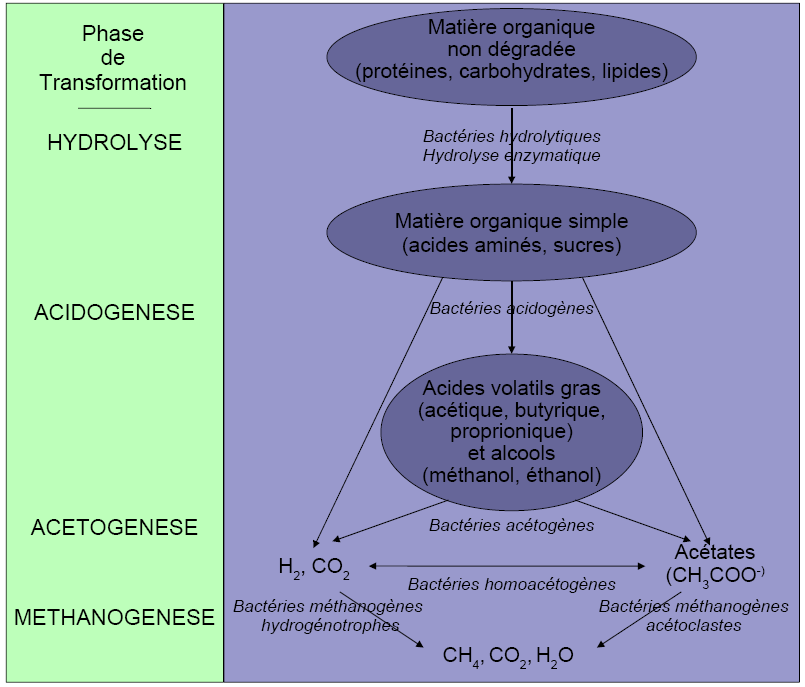
\includegraphics[scale=0.3]{schema/process_biologique_methanisation_et_biogaz.png}
		\end{figure}
\end{frame}
 \begin{frame}{Biométhanisation}
	\begin{columns}
		
		\begin{column}{0.35\textwidth}
		Composition:
			\begin{itemize}
			\item 50 à \unit{70}{\%} de \ce{CH4}
			\item 15 à \unit{45}{\%} de \ce{CO2}
			\item  \unit{5}{\%} de \ce{H2O}
			\item 0 à \unit{2}{\%} de \ce{H2S}
			\item impuretés (négligeable)
			\end{itemize}
		\end{column}
		\begin{column}{0.50\textwidth}
		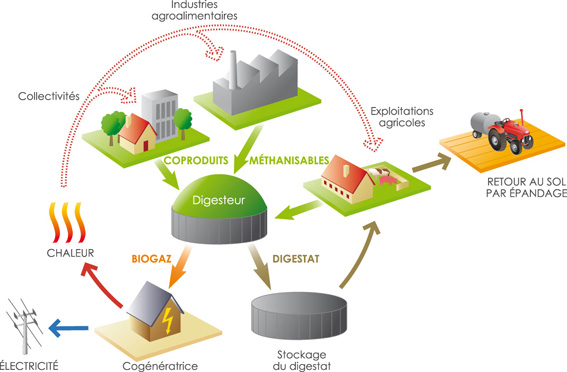
\includegraphics[scale=0.3]{schema/installationdebiomethanisation_Ledjo.jpg}
		\end{column}
	\end{columns}
\end{frame}
\begin{frame}{Biogaz}
	\begin{columns}
		
		\begin{column}{0.40\textwidth}		
		Avantages:
			\begin{itemize}
			\item Ecologique 
				\begin{itemize}
				\item \ce{CO2}
				\item \ce{CH4}
				\end{itemize}
			\item Réduction des problèmes liés au transport
			\item Réduction de la consommation d'énergie
			\end{itemize}
		\end{column}
		\begin{column}{0.40\textwidth}
		Faisabilité:
		\begin{itemize}
		\item Région wallonne : environ \unit{485.33 \cdot 10^3}{t/an} de \ce{CH4} provenant de biogaz (potentiel)
		\item \unit{1500}{t/j} de \ce{NH3} $\Longrightarrow$ \unit{258.7 \cdot 10^3}{t/an} de \ce{CH4}
		\item Représente 53.3 \%  de la production en biométhane wallonne
		\item Impossibilité de remplacer le gaz naturel totalement par du biogaz
		\end{itemize}
		\end{column}
	\end{columns}
\end{frame}

\begin{frame}{Chlamydomonas reinhardtii : l'hydrogène du futur ?}
	\begin{columns}
		\begin{column}{0.40\textwidth}
		\begin{figure}
		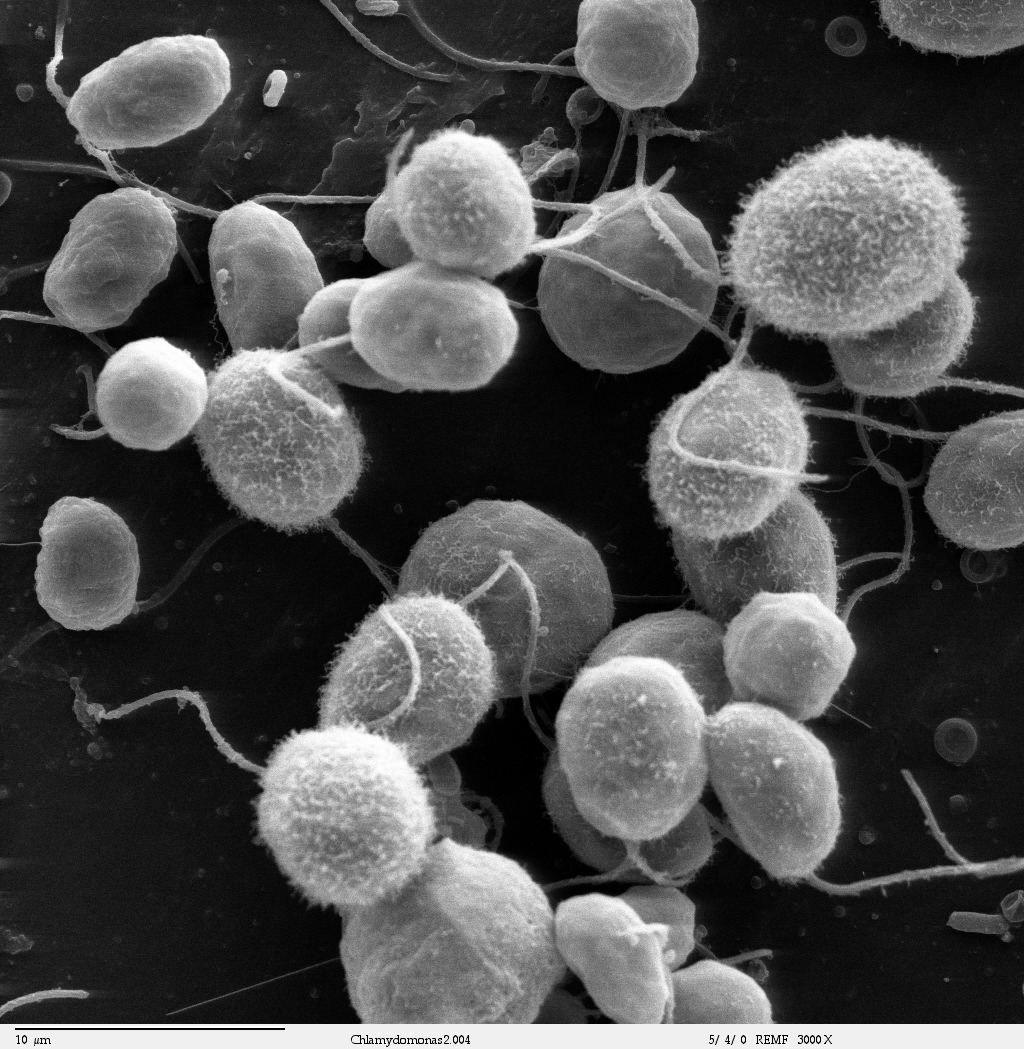
\includegraphics[scale=0.14]{schema/Chlamydomonas.jpg}
		\end{figure}
		
		\end{column}
		\begin{column}{0.40\textwidth}
		Mécanisme de production d'hydrogène découvert en 1990 à l'Université de Californie à Berkeley.\\[1em]
		
		Privée de soufre, C.\;reinhardtii produit de l'hydrogène au lieu d'oxygène.
		\end{column}
	\end{columns}
\end{frame}
\begin{frame}{Avantages de la production d'hydrogène par des algues}
	\begin{columns}
		\begin{column}{0.40\textwidth}
		\begin{itemize}
		\item Pas d'impact \ce{CO2} direct
		\item Source renouvelable et extensible d'hydrogène
		\item Avantages de l'hydrogène (combustion propre, haute densité d'énergie)
		\end{itemize}
		\end{column}
		\begin{column}{0.40\textwidth}
		\begin{figure}
		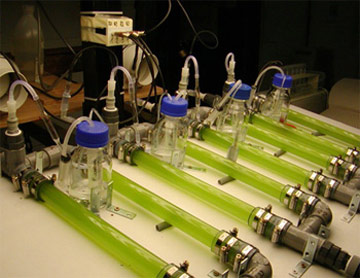
\includegraphics[scale=0.4]{schema/algues_labo.jpg}
		\end{figure}
		
		\end{column}
	\end{columns}
\end{frame}
\begin{frame}{Prédictions}
	    Sur base des recherches actuelles, nous pouvons extrapoler :
	\begin{columns}
		\begin{column}{0.40\textwidth}
		\begin{itemize}
		\item Pour produire \unit{1500}{\ton\per j} de \ce{NH3}, il nous faut \unit{266}{\ton\per j} d'hydrogène
		\item En Belgique, cela nécessite \unit{200}{\kilo\meter\squared}
		\item $\approx \unit{0.6}{\%}$ surface de la Belgique
		\end{itemize}
		\end{column}
		\begin{column}{0.40\textwidth}
		Coût de l'hydrogène
		\begin{itemize}
		\item À partir d'algues : entre \unit{1}{}et \unit{6}{USD\per\kilogram}
		\item À partir de gaz naturel : \unit{\sim 3}{USD\per\kilogram}
		\end{itemize}
		\end{column}
	\end{columns}
\end{frame}
\begin{frame}{En conclusion}
    \begin{center}
	    Beaucoup de potentiel mais aucune réelle alternative au gaz naturel aujourd'hui\\[1em]
	    $\implies$ investir pour le futur.
    \end{center}
\end{frame}

\begin{frame}
\begin{center}
Slides supplémentaires
\end{center}
\end{frame}
\begin{frame}{Analyse du progrès du groupe}

		\begin{center}
		Organisation du groupe:
			\begin{itemize}
			\item Utilisation de Github.
			\item Planification par écrit des tâches.
			\item Réservation de Locaux en BST.
			\end{itemize}
		\end{center}

\end{frame}

\begin{frame}[allowframebreaks]{Le biogaz en Wallonie}
		\begin{center}
\scalebox{0.8}{
\begin{tabular}{|c|c|c|}
\hline 
 & Gisement ($\unit{10^6}{t}$) & Productivité ($\unit{}{m^3_{\ce{CH4}}/t)}$\\ 
\hline 
Effluents agricoles & 18.2 & 31.5  \\ 
\hline 
Résidus agro-industriels & 1.15 & 60 \\ 
\hline 
Résidus organiques ménagers + déchets verts & 1 & 65\\ 
\hline 
Boues de STEP& 0.07 & 230 \\ 
\hline 
Total & 20.42 & \\ 
\hline 
\end{tabular} 
}
\end{center}


A partir de ces données, nous pouvons faire un estimation de la production de biométhane en Wallonie:

$$18.2\cdot \num{e6} \cdot 31.5 + 1.15\cdot \num{e6} \cdot 60 + 1\cdot \num{e6} \cdot 65 + 0.07\cdot \num{e6} \cdot 230 = \unit{729.4\cdot \num{e6}}{m^3}$$ en sachant que le masse volumique du \ce{CH4} est de \unit{0.6790}{kg/m^3},
on obtient que la combinaison de ces 4 ressources, nous engendre une production de $\unit{485.33 \cdot \num{e3}}{t/an}$ de \ce{CH4}.

Comme nous avons besoin de \unit{708.76}{t/day} de \ce{CH4}, il nous faut \unit{258697.5}{T/ans} de \ce{CH4}. Ce qui équivaut à \unit{53.3}{\%} de la production de biométhane en Wallonie.

\end{frame}

\begin{frame}{Flowsheet}
\begin{center}
\resizebox{6cm}{6cm}{
	\newpage
\section{Flowsheet}\label{appendix:flowsheet}

\tikzstyle{decision} = [diamond, draw, fill=blue!20,
    text width=4.5em, text badly centered, node distance=3cm, inner sep=0pt]
\tikzstyle{block} = [rectangle, draw, fill=blue!20,
    text width=14em, text centered, rounded corners, minimum height=4em, minimum width=15em, node distance=3cm]
\tikzstyle{block2} = [rectangle, draw, fill=red!20,
    text width=14em, text centered, rounded corners, minimum height=4em, minimum width=15em, node distance=3cm]
\tikzstyle{line} = [draw, -latex']
\tikzstyle{cloud} = [draw, ellipse,fill=red!20, node distance=3cm,
    minimum height=2em]

\begin{center}
	%\begin{tikzpicture}[thick,scale=0.6, every node/.style={scale=0.6}]
	\begin{tikzpicture}[node distance = 3cm, auto]
	    % Place nodes
	    \node [block] (RefPrim) {\textbf{Réformage primaire}(Réformage à vapeur de \ce{CH_4}) $$\ce{CH_4 + H_2O <=> CO + 3H_2}$$ $$\ce{CO + H2O <=> H2 + CO2}$$ \textit{Equilibre à T (sortie)} };
	    \node [block2, left of=RefPrim, node distance=7cm] (Four) {\textbf{Four} \\ Combustion de \ce{CH_4} \\ \textit{Irreversible et complète}};
	    \node [block, below of=RefPrim, node distance=3.5cm] (RefSec) {\textbf{Réformage secondaire} $$\ce{2CH4 + O2 -> 2CO + 4H2}$$ \textit{Considérée comme irréversible et complète à la fin.}};
	    \node [block, below of=RefSec, node distance=3.5cm] (Reacteur) {\textbf{Réacteurs Water-Gas-Shift} $$\ce{CO + H2O -> CO2 + H2}$$ \textit{Considérée comme complète à la fin.} };
	    \node [block, below of=Reacteur, node distance=3.5cm] (AbsComp) {\textbf{Absorption de \ce{CO2} et compression} (séparation d'\ce{H2 O}) \\ \textit{Considérées complètes.}};
	    \node [block, below of=AbsComp, node distance=3.5cm] (Synth) {\textbf{Synthèse d'\ce{NH3} et séparation} $$\ce{N2 + 3H2 <=> 2NH3}$$ \textit{Considérées complètes.}};
	    \node [right of =AbsComp, node distance=6cm] (nothing1){};
	    \node [below of =Synth] (nothing2){};
	    \node [left of =RefSec, node distance=6cm] (nothing3){};
	    \node [above of =RefPrim, node distance=4cm] (nothing4){};
	    \node [left of =Four, node distance=5cm] (nothing5){};
	    \node [above of =Four, node distance=4cm] (nothing6){};
	    % Draw edges
	    \path [line] (RefPrim) -- node {\ce{CH4}, \ce{H2O}}(RefSec);
	    \path [line] (Four) -- node {ENERGY} (RefPrim);
	    \path [line] (RefSec) -- (Reacteur);
	    \path [line] (Reacteur) -- node {\ce{CO2(g) + H2(g)}} (AbsComp);
	    \path [line] (AbsComp) -- (Synth);
	    \path [line] (AbsComp) -- node {\ce{CO2(g)}, \ce{H2O(g)}}(nothing1);
	    \path [line] (Synth) -- node {\ce{NH3(l)}, \ce{Ar(g)}}(nothing2);
	    \path [line] (nothing3) -- node {\ce{O2(g)}, \ce{N2(g)},\ce{Ar(g)}}(RefSec);
	    \path [line] (nothing4) -- node {\ce{CH4(g)}, \ce{H2 O(l)}}(RefPrim);
	    \path [line] (Four) -- node {\ce{CO2+2H2O}} (nothing5);
	    \path [line] (nothing6) -- node {\ce{CH4(g), H2O(l)}} (Four);
	\end{tikzpicture}
\end{center}
}
\end{center}
\end{frame}

\end{document}